\chapter{BTOR2 Frontend in Theta}

\section{Motivation}
The goal of this project is to provide a direct BTOR2 frontend for the Theta model checker, translating BTOR2 models into Theta's XCFA representation. While the existing tool Btor2C translates BTOR2 into C for use with software verifiers, this detour might introduce unnecessary complexity and limits optimization opportunities.\cite{btor2c} A native frontend will hopefully enable a more efficient, faster, and easier-to-optimize verification flow by eliminating intermediate representations.

\section{BTOR2XCFA transformation}
The transformation from BTOR2XCFA is the core of this frontend and represents the majority of the work. BTOR2 models consist of a sequence of node declarations (like \verb*|state|, \verb*|init|, \verb*|next|, \verb*|and|, \verb*|or|, \verb*|eq|, etc.), which define a transition system. These nodes must be carefully mapped into a control-flow structure in Theta.~\cite{theta}{btor2}

\begin{figure}
  \centering
  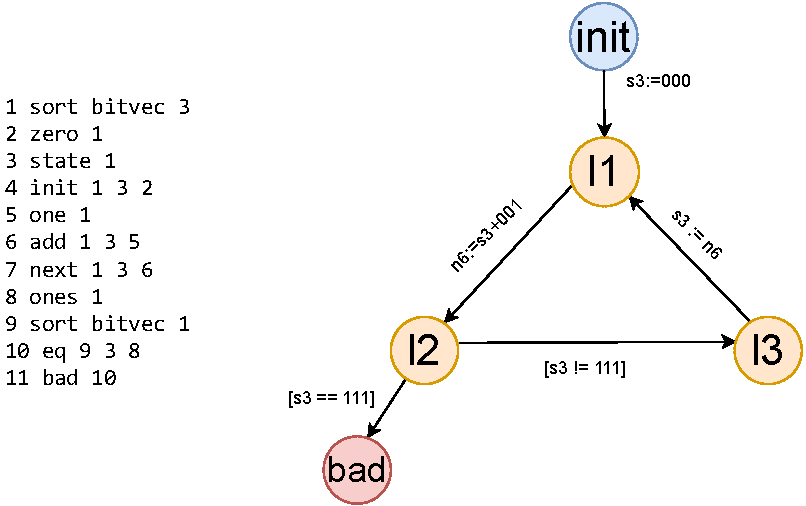
\includegraphics[width=0.8\textwidth]{figures/count2_cfa_code.pdf}
  \caption{ Transformation of a simple BTOR2 circuit to XCFA }
  \label{fig:count2_cfa_code}
\end{figure}

Figure~\ref{fig:count2_cfa_code} presents a minimal example of how a BTOR2 model can be transformed into an Extended-Control-Flow Automata (XCFA), as used in the Theta model checker. On the left-hand side, we see a BTOR2 description of a simple counter system, while the right-hand side shows its corresponding XCFA representation. This example serves to demonstrate the key steps in the transformation process from BTOR2's flat instruction-based semantics to Theta's control-flow-based representation.

In the BTOR2 model, the system is defined over a single 3-bit state variable named s3. The model begins by declaring the 3-bit bitvector sort (line 1), followed by constants such as zero and one. The state variable s3 is initialized to zero (line 4), representing the starting point of the system. The behavior of the system is defined by incrementing the state variable on each transition. This is done through the add operation (line 6), which adds 1 to the current state (s3 + 1), and the next assignment (line 7), which updates s3 to this new value. Finally, a bad state is defined (line 11), which is triggered when the value of s3 reaches its maximum possible value, 111 in binary (i.e., 7 in decimal).

The XCFA representation on the right visualizes this transition system as a graph of control locations and edges labeled with operations or guards. The init node is the entry point of the system, where s3 is initialized to 000. The control then proceeds to location l1, where the arithmetic operation n6 := s3 + 1 is prepared. From l1, the automata moves to location l2, where a conditional check determines whether s3 has reached the value 111. If the condition is true, the system transitions into the bad location, signaling that the safety property has been violated. Otherwise, it proceeds to location l3, where the state variable is updated with the new value (s3 := n6), and control returns to l1, effectively looping the counter.

This small example illustrates the straightforward nature of the BTOR2XCFA transformation for simple systems. Each BTOR2 instruction maps to a specific element in the XCFA: init maps to the initial control edge, next becomes a state update assignment, and bad becomes a conditional edge to an error location. Importantly, this mapping allows us to express the semantics of the bitvector-based transition system using the higher-level control-flow structure supported by Theta. It also demonstrates how Theta can be used to verify safety properties directly on the XCFA, without the need to lower the input to a general-purpose programming language like C.

As a pedagogical example, this model captures the essence of the transformation process and highlights how simple bitvector logic can be interpreted in a control-flow context. It also sets the stage for handling more complex constructs and optimizations in larger BTOR2 systems.

\section{Implementation}
The implementation of the BTOR2 frontend in Theta is centered around a \textit{visitor pattern}, which allows us to traverse the BTOR2 program and categorize each node based on its role—such as constants, statefuls, operations, or properties. Using this structure, we first collect all nodes into separate arrays during a preprocessing step. Once categorized, the transformation into an XCFA proceeds in stages: each node is mapped to a corresponding XCFA location, and transitions are added to reflect the behavior of the system.

The XCFA construction follows a fixed order: we begin by inserting \textit{init edges} that define the system's initial state, then add \textit{input values} and \textit{operation edges} that represent logical or arithmetic behavior. Next, we encode \textit{bad state properties} as conditional transitions to a dedicated \verb*|bad| location, and finally insert \textit{next state updates} that drive the system's evolution. A notable implementation detail is handling negation, which BTOR2 represents using bit tricks (e.g., two's complement). Since this encoding isn't clearly documented, custom logic was required to interpret these correctly. The transformation uses \textbf{ANTLR} for parsing, and each node type is handled modularly, ensuring a clear and extensible pipeline for future enhancements.\cite{antlr}

\section{Current limitations}
Although the BTOR2 frontend for Theta is functional, there are several limitations that currently restrict its completeness and expressiveness. Some BTOR2 operators—such as overflow-detecting predicates—are not yet supported, as Theta lacks native constructs for these. Additionally, the frontend does not currently handle array operations, which would be essential for modeling more complex hardware components. These are left for future development.

At present, the frontend supports only \texttt{bad} properties, which represent safety requirements; i.e., properties that state ``something bad should never happen.'' While Theta has support for \emph{liveness} properties (``something good should eventually happen''), the translation of such specifications from BTOR2 would require more sophisticated modeling techniques and is therefore not yet implemented.
 
\section{Prelimanary results}
Initial experiments show promising results. The BTOR2XCFA transformation works reliably for small to medium-sized benchmarks. The generated XCFAs maintain semantic consistency with the original models, and Theta is able to verify the transformed models efficiently in many cases. These early successes indicate that the approach is viable and has potential for further extension.

% Please add the following required packages to your document preamble:
% \usepackage{booktabs}
\begin{table}[h]
\centering
\begin{tabular}{@{}lllll@{}}
\toprule
Category                     & Count & CPU Time (s) & Wall Time (s) \\ \midrule
All results                           & 5277  & 19100        & 20400         \\
Local summary                         & -     & 18800        & 21900         \\
\quad Correct results                      & 22    & 434          & 437           \\
\quad\quad Correct true                     & 2     & 3.79         & 4.60          \\
\quad\quad Correct false                    & 20    & 430          & 432           \\
\quad Incorrect results                    & 4     & 85.9         & 86.1          \\
\quad\quad Incorrect true                   & 2     & 3.52         & 3.58          \\
\quad\quad Incorrect false                  & 2     & 82.4         & 82.5          \\
Score (of 5277 tasks, max score: 8557)  & -72   & -            & -             \\ \bottomrule
\end{tabular}
\caption{ Summary of results, times, and scores }
\label{table:summary}
\end{table}

A small benchmark summary in Table~\ref{table:summary} shows that the transformation pipeline performs well and that Theta can complete verification tasks quickly. While these are preliminary outcomes, they confirm that the architecture of the frontend is sound and offer motivation for continued work.

% Please add the following required packages to your document preamble:
% \usepackage{booktabs}
% \usepackage{graphicx}
\begin{table}[h]
\resizebox{\textwidth}{!}{%
\begin{tabular}{@{}lll@{}}
\toprule
Status                                           & Tasks (pieces) & (Possible) Causes                                     \\ \midrule
Incorrect true                                   & 2              & No operations                                         \\
Incorrect false                                  & 2              & Too many havocs                                       \\
TIMEOUT                                          & 99             & 60s limit                                             \\ 
OUT OF MEMORY                                    & 95             & 1 GB limit                                            \\
ERROR ( generic error, before parsing finished)  & 792            & "Not yet implemented"                                 \\
ERROR (frontend failed, before parsing finished) & 4265           & NumberFormatException (decimal numbers, minuses etc.) \\ \bottomrule
\end{tabular}%
}
\caption{ Summary of errors }
\label{table:errors}
\end{table}

However, a detailed error analysis, summarized in Table~\ref{table:errors}, highlights several limitations and points to areas for improvement. A significant number of tasks (4265 out of 5277) failed due to frontend errors before parsing even finished. Most of these were caused by a NumberFormatException, likely stemming from the handling of decimal numbers, negative values, or other unsupported formats. Additionally, 792 tasks encountered a generic error marked as "Not yet implemented," indicating missing functionality in the frontend parser or transformer.

Resource limitations also affected the results: 99 tasks hit the 60-second timeout threshold, and 95 were terminated due to exceeding the 1 GB memory limit. These point to performance bottlenecks that may be mitigated with optimizations in the transformation or verification process.

A small number of tasks (4) produced incorrect results, evenly split between incorrect true and false verdicts. The causes identified include missing operations and an excessive number of havoc operations, suggesting that while the core transformation is generally correct, it still needs refinement to handle edge cases robustly.

Despite these challenges, the toolchain demonstrated correctness on 22 benchmarks with a balanced distribution between true and false results, and verification times were consistently low. These outcomes support the feasibility of the BTOR2XCFA pipeline and provide a solid foundation for future enhancements in error handling, performance, and language coverage.

\section{Conclusion}
This work introduced a BTOR2 frontend for the Theta model checker, enabling the transformation of BTOR2 hardware models into (extended-)control-flow automata (XCFA). The translation preserves key semantics of the input model and focuses on supporting safety properties. Using a visitor pattern and ANTLR for parsing, the implementation is modular and maintainable, allowing for flexible extension in the future.

Despite the current limitations—such as incomplete operator support and the absence of liveness translation—the foundation is robust. The frontend already handles basic BTOR2 programs effectively, and serves as a solid basis for building more advanced features.

\subsection{Future work}
There are several directions for further development. Supporting overflow-detecting operators and other complex BTOR2 constructs is a priority. Translation of liveness properties into Theta is another significant milestone that requires more sophisticated temporal modeling.

Witness generation is also crucial, especially for participation in hardware model checking competitions (HWMCC). Furthermore, broader benchmarking and debugging are needed to evaluate robustness and correctness. Finally, adding optimization passes on the generated XCFA will improve performance and scalability. With these improvements, the frontend can evolve into a competitive and comprehensive solution for hardware verification within Theta.
